Ao aplicar um impulso nas entradas do sistema modelado para representar o quadrotor, os estados relacionados à altitude e atitude divergem, como é mostrado na Figura \ref{fig:uncontrolled}. Nota-se que a divergência dos ângulos ($\phi$ e $\theta$) é linear, mostrando que o impulso aplicada na entrada é, de fato, a aceleração do sistema sobre essas saídas. Já a variável relacionada à atitude ($z$) decai em parábola, devido à ação da gravidade, o que indica que o impulso é também, de fato, uma aceleração extra do sistema no eixo $z$, como a modelagem adotada propõe.

% Sistema nao controlado
\begin{figure}[!htb]
    \centering
    \caption{Divergência das variáveis relacionadas a altitude e atitude quando o sistema é submetido a um impulso nas entradas}
    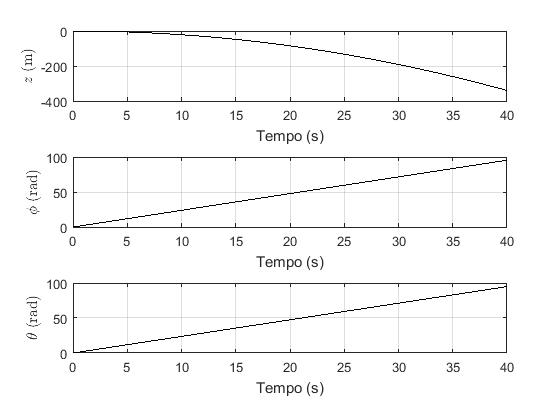
\includegraphics[width=0.8\textwidth]{./04-figuras/resultados/novos/uncontrolled}
    \label{fig:uncontrolled}
\end{figure}

Com estes resultados, fica clara a necessidade de controladores para estabilizar o sistema. Os próximos resultados mostram a resposta do sistema estabilizado pelos controladores fuzzy e neuro-fuzzy projetados.